\documentclass[final,3p,fleqn, 10pt]{elsarticle}
% Recommended, but optional, packages for figures and better typesetting:
\makeatletter
\def\ps@pprintTitle{%
 \let\@oddhead\@empty
 \let\@evenhead\@empty
 \def\@oddfoot{}%
 \let\@evenfoot\@oddfoot}
\makeatother
\usepackage[capposition=top]{floatrow}
\usepackage[utf8]{inputenc}%(only for the pdftex engine)
%\RequirePackage[no-math]{fontspec}%(only for the luatex or the xetex engine)
 \usepackage{url} 
%\usepackage[margin=1in]{geometry} 
\usepackage{setspace}

\setstretch{1.15}
 
% Packages from D-LATE preamble (potentially useful and not obviously covered by dgruyter)
\usepackage{microtype}
\usepackage{graphicx} % Already used by dgruyter but good to ensure
\usepackage{subfigure} % For subfigures, if any are added later
%\usepackage{subcaption}
\usepackage{booktabs} % For professional tables
\usepackage{natbib} % For bibliography management
\usepackage{amsmath} % dgruyter likely includes it, but explicit is safe
\usepackage{amssymb} % dgruyter likely includes it
\usepackage{mathtools} % Extends amsmath
\usepackage{amsthm} % For theorems, dgruyter might have its own, but this is standard
\usepackage{bm} % For \mathbbm{1} (bold math for indicator) - or use dsfont
\usepackage{dsfont} % Alternative for \mathds{1} if \mathbbm{1} is problematic
\usepackage[capitalize,noabbrev]{cleveref} % For smart cross-referencing

% Custom commands and theorem environments from D-LATE preamble
\usepackage{enumitem} % Though lists will be converted to paragraphs
\usepackage{color} % Unlikely needed for final submission

\newcommand{\indep}{\rotatebox[origin=c]{90}{$\models$}}
\newcommand\Norm {\mathcal{N}}
\newcommand\E {\mathbb{E}}
\newcommand\Expect{\E}
% \renewcommand\Re{\R} % \R is already defined below, avoid redefinition conflict if possible
\newcommand\bs {\boldsymbol}
\newcommand\bPsi {\bs{\psi_u}}
% \newcommand\X {\mathcal{X}} % \cX is defined below
\newcommand\bxi {\bs{\xi}}
\newcommand\z {\mathtt z}
\newcommand\Var {\ensuremath{\mathrm{Var}}}
\newcommand\Cov {\ensuremath{\mathrm{Cov}}}
\newcommand\sign {\ensuremath{\operatorname{\mathrm{sign}}}}
\newcommand\sam {\ensuremath{\operatorname{\mathrm{sam}}}}
\newcommand\zu {\mathfrak{z}}
\newcommand*{\defeq}{\stackrel{\textup{def}}{=}}
\newcommand*{\eqdef}{\stackrel{\textup{def}}{=}}
\newcommand\range {\ensuremath{\operatorname{\mathrm{range}}}}
\newcommand\mynull {\ensuremath{\operatorname{\mathrm{null}}}}
\newcommand\rank {\ensuremath{\operatorname{\mathrm{rank}}}}
\newcommand\krank {\ensuremath{\operatorname{\mathrm{krank}}}}
\newcommand\spark {\ensuremath{\operatorname{\mathrm{spark}}}}
\newcommand\conv {\ensuremath{\operatorname{\mathrm{conv}}}}
\newcommand\poly {\ensuremath{\operatorname{\mathrm{poly}}}}
\newcommand\nnz {\ensuremath{\operatorname{\mathrm{nnz}}}}
\newcommand\tr {\ensuremath{\operatorname{\mathrm{tr}}}}
\newcommand\diag {\ensuremath{\operatorname{\mathrm{diag}}}}
\newcommand\ind {\mathds{1}} % Using \mathds from dsfont
% \renewcommand\Re{\mathbb{R}} % \R is defined as \mathbb{R} below

%Calligraphic Shorthands
\newcommand{\cA}{\mathcal{A}}
\newcommand{\cB}{\mathcal{B}}
\newcommand{\cC}{\mathcal{C}}
\newcommand{\cD}{\mathcal{D}}
\newcommand{\cE}{\mathcal{E}}
\newcommand{\cF}{\mathcal{F}}
\newcommand{\cG}{\mathcal{G}}
\newcommand{\cH}{\mathcal{H}}
\newcommand{\cI}{\mathcal{I}}
\newcommand{\cJ}{\mathcal{J}}
\newcommand{\cL}{\mathcal{L}}
\newcommand{\cM}{\mathcal{M}}
\newcommand{\cN}{\mathcal{N}} % Already \Norm
\newcommand{\cO}{\mathcal{O}}
\newcommand{\cP}{\mathcal{P}}
\newcommand{\cQ}{\mathcal{Q}}
\newcommand{\cR}{\mathcal{R}}
\newcommand{\cS}{\mathcal{S}}
\newcommand{\cT}{\mathcal{T}}
\newcommand{\cU}{\mathcal{U}}
\newcommand{\cV}{\mathcal{V}}
\newcommand{\cW}{\mathcal{W}}
\newcommand{\cX}{\mathcal{X}}
\newcommand{\cY}{\mathcal{Y}}
\newcommand{\cZ}{\mathcal{Z}}

%Blackboard Bold Shorthands
\newcommand{\bE}{\mathbb{E}}
\newcommand{\bP}{\mathbb{P}}
\newcommand{\N}{\mathbb{N}}
\newcommand{\R}{\mathbb{R}}
\newcommand{\Z}{\mathbb{Z}}
% \newcommand{\F}{\mathbb{F}} % \F is not used in D-LATE main text
\newcommand{\GG}{\mathbb{G}}
\newcommand{\B}{\mathbb{B}}
% \newcommand{\V}{\mathbb{V}} % \V is not used in D-LATE main text
\newcommand{\Nbb}{\mathbb{N}}
\newcommand{\Ecal}{\mathcal{E}}
\newcommand{\Mcal}{\mathcal{M}}
\newcommand{\KL}{\mathrm{KL}}
\newcommand{\kl}{\mathrm{kl}}
\newcommand{\Alt}{\mathrm{Alt}}
\newcommand{\Local}{\mathrm{Local}}
\newcommand{\annot}[2]{\underbrace{#1}_{\text{#2}}}

%% 1 
% \newcommand{\1}{\mathbbm{1}} % Replaced by \ind using \mathds{1}

%Probability Shorthands
\newcommand{\norm}[2]{\mathcal{N}\left(#1,#2\right)}
\newcommand{\bet}[2]{\text{Beta}\left(#1,#2 \right)}
\newcommand{\muhat}{\widehat{\mu}}
\newcommand{\bmu}{\bm{\mu}}
\newcommand{\K}{\mathrm{KL}} % Already defined
\newcommand{\Kb}{\mathrm{K}}
\newcommand{\iid}{ \stackrel{\mathrm{i.i.d}}{\sim} }
\newcommand{\btau}{\mathbf{y}}
\newcommand{\bX}{\mathbf{X}}
\newcommand{\bpi}{\pmb{\pi}}
\newcommand{\bh}{\mathbf{\pi}}
\newcommand{\bA}{\mathbf{A}}
\newcommand{\bB}{\mathbf{B}}
\newcommand{\smallo}{{\scriptscriptstyle\mathcal{O}}} %
\newcommand{\bo}{\mathbf{0}}
\newcommand{\by}{\mathbf{y}}
\newcommand{\bG}{\mathbb{G}} % Already \GG
\def\Holder{{H\"{o}lder}}
\newcommand{\bu}{\mathbf{u}}
\def\Cramer{Cram\'{e}r}
\newcommand{\bU}{\mathbf{U}}
\newcommand{\nhs}{n^{\mathrm{hst}}}
\newcommand{\fix}{\mathrm{fix}}
\newcommand{\nev}{n^{\mathrm{evl}}}
\newcommand{\EB}{\mathrm{EB}}
\newcommand{\para}{\mathrm{para}}
\newcommand{\bN}{\mathcal{N}} % Already \Norm
\newcommand{\oO}{\mathcal{O}} % Already \cO
\newcommand{\ch}{\mathcal{H}} % Already \cH
\newcommand{\bigO}{\mathcal{O}} % Already \cO
\newcommand{\cj}{\mathcal{J}} % Already \cJ
\newcommand{\bv}{\mathbf{v}}
\newcommand{\bw}{\mathbf{w}}
\newcommand{\CR}{\mathrm{CR}}
\newcommand{\noo}{\mathrm{no}}
\newcommand{\te}{\mathrm{te}}
\newcommand{\VC}{\mathrm{VC}}
\newcommand{\case}{\mathrm{case}}
\newcommand{\buu}{\mathbf{u}} % Already \bu
\renewcommand{\P}{\mathbb{P}} % Already \bP
\newcommand{\Gn}{\mathbb{G}_{n}}
\newcommand{\hP}{\mathbb{P}_n}
\newcommand{\hG}{\mathbb{G}} % Already \GG
\newcommand{\Op}{\mathrm{O}_{p}}
\newcommand{\op}{\mathrm{o}_{p}}
\newcommand{\Pa}{\mathrm{Pa}}
% \newcommand{\pa}{\mathrm{\pa}} % \pa is not defined, might be typo for Pa
\newcommand{\mI}{\mathcal{I}} % Already \cI
\newcommand{\calh}{\mathcal{H}} % Already \cH
\newcommand{\rI}{\mathrm{I}}
\newcommand{\var}{\mathrm{var}} % Standard, but \Var is also defined
\newcommand{\cov}{\mathrm{cov}} % Standard, but \Cov is also defined
\newcommand{\rE}{\mathrm{E}} % Standard, but \E is also defined
\newcommand{\thpol}{\pi^{\theta}}
\newcommand{\thhatpol}{\pi^{\widehat{\theta}}}
\newcommand{\rvar}{\mathrm{var}} % Already \var
\newcommand{\Asmse}{\mathrm{Asmse}}
\newcommand{\dml}{\mathrm{dml}}
\newcommand{\dm}{\mathrm{dm}}
\newcommand{\rD}{\mathrm{d}}
\newcommand{\rd}{\mathrm{d}} % Already \rD
\newcommand{\bbN}{\mathbb{N}} % Already \N
\newcommand{\prns}[1]{\left(#1\right)}
\newcommand{\braces}[1]{\left\{#1\right\}}
\newcommand{\bracks}[1]{\left[#1\right]}
\newcommand{\sumT}{\sum_{t=0}^T}
\newcommand{\abs}[1]{\left|#1\right|}
\newcommand{\Rl}{\mathbb{R}} % Already \R
\newcommand{\epol}{\pi^\mathrm{e}}
\newcommand{\bpol}{\pi^\mathrm{b}}
\newcommand{\pre}{\mathrm{pre}}
\newcommand{\tmle}{\mathrm{tmle}}
\newcommand{\ipw}{\mathrm{ipw}}
\newcommand{\prepi}[1]{d_0 \times #1}
\newcommand{\ini}{p_{\mathrm{ini}}}
\newcommand{\opera}{p_{\mathrm{op}}}
\newcommand{\inipi}[1]{p_{\mathrm{ini}, #1}}
\newcommand{\magd}[1]{\left\|#1\right\|}
\newcommand{\Rfrak}{\mathfrak{R}}
\newcommand{\Fcal}{\mathcal{F}} % Already \cF
\newcommand{\Scal}{\mathcal{S}} % Already \cS
\newcommand{\Acal}{\mathcal{A}} % Already \cA
\newcommand{\Xcal}{\mathcal{X}} % Already \cX
\newcommand{\Wcal}{\mathcal{W}} % Already \cW
\newcommand{\RR}{\mathbb{R}} % Already \R
\newcommand{\Qcal}{\mathcal{Q}} % Already \cQ
\newcommand{\Vcal}{\mathcal{V}} % Already \cV
\newcommand{\Gcal}{\mathcal{G}} % Already \cG
\newcommand{\Rcal}{\mathcal{R}} % Already \cR
\newcommand{\Zcal}{\mathcal{Z}} % Already \cZ
\newcommand{\bzero}{\mathbf{0}} % Already \bo
\newcommand{\Lcal}{\mathcal{L}} % Already \cL
\newcommand{\Lw}{L_{\mathrm{w}}}
\newcommand{\Lwn}{L_{\mathrm{w},n}}
\newcommand{\Lq}{L_{\mathrm{q}}}
\newcommand{\Lqn}{L_{\mathrm{q},n}}
\newcommand{\hatw}{\widehat{w}}
\newcommand{\hatwn}{\widehat{w}_n}
\newcommand{\hatq}{\widehat{q}}
\newcommand{\hatqn}{\widehat{q}_n}
\newcommand{\oder}{\mathrm{o}} % Already \op
\newcommand{\vecsigma}{\vec{\sigma}}
\newcommand{\vecmu}{\vec{\mu}}
\newcommand{\AltDelta}{\Alt_\Delta}
\newcommand{\tildesigma}{\sqrt{\widetilde{V}^a}}
\newcommand{\ep}{\hfill $\Box$}
\newcommand{\bepsilon}{{\mbox{\boldmath$\epsilon$}}}
\newcommand{\RN}[1]{%
  \textup{\uppercase\expandafter{\romannumeral#1}}%
}
\newcommand{\SDelta}{\mathcal{S}(\Delta)}
\newcommand*\interior[1]{#1^{\mathsf{o}}}
\newcommand{\dvert}{\mathrm{d}} % Already \rD

% THEOREM Environments (dgruyter.sty might define its own, these are from D-LATE preamble)
% It's safer to let dgruyter.sty handle theorem environments if it does.
% If not, these can be uncommented. For now, assume dgruyter handles them or use its specific versions.
% \theoremstyle{plain}
% \newtheorem{theorem}{Theorem}[section]
% \newtheorem{proposition}[theorem]{Proposition}
% \newtheorem{lemma}[theorem]{Lemma}
% \newtheorem{corollary}[theorem]{Corollary}
% \theoremstyle{definition}
% \newtheorem{definition}[theorem]{Definition}
% \newtheorem{assumption}[theorem]{Assumption} % D-LATE uses this
% \theoremstyle{remark}
% \newtheorem{remark}[theorem]{Remark}

% JCI template uses \theoremstyle{dgthm} \newtheorem{thm}{Theorem} etc.
% I will use the D-LATE Assumption environment style as it's specifically used.
\theoremstyle{definition} % Or \theoremstyle{dgdefinition} if dgruyter has it
\newtheorem{assumption}{Assumption}[section] % Match D-LATE paper's usage
\newtheorem{theorem}{Theorem}[section] % Match D-LATE paper's usage for consistency

\begin{document}
\begin{frontmatter}
\title{Rethinking Distributional IVs: KAN-Powered D-IV-LATE \& Model Choice}
\author{Charles Shaw. \\This version \today}
\date{this version \today}

  \begin{abstract}
The double/debiased machine learning (DML) framework has become a cornerstone of modern causal inference, allowing researchers to utilise flexible machine learning models for the estimation of nuisance functions without introducing first-order bias into the final parameter estimate. However, the choice of machine learning model for the nuisance functions is often treated as a minor implementation detail. In this paper, we argue that this choice can have a profound impact on the substantive conclusions of the analysis. We demonstrate this by presenting and comparing two distinct Distributional Instrumental Variable Local Average Treatment Effect (D-IV-LATE) estimators. The first estimator leverages standard machine learning models like Random Forests for nuisance function estimation, while the second is a novel estimator employing Kolmogorov-Arnold Networks (KANs). We establish the asymptotic properties of these estimators and evaluate their performance through Monte Carlo simulations. An empirical application analysing the distributional effects of 401(k) participation on net financial assets reveals that the choice of machine learning model for nuisance functions can significantly alter substantive conclusions, with the KAN-based estimator suggesting more complex treatment effect heterogeneity. These findings underscore a critical "caveat emptor". The selection of nuisance function estimators is not a mere implementation detail. Instead, it is a pivotal choice that can profoundly impact research outcomes in causal inference.

\vspace{10pt}
Keywords Distributional Treatment Effects, Instrumental Variables, Kolmogorov-Arnold Networks, Machine Learning, Causal Inference, Endogeneity, Nuisance Functions, Model Choice
\end{abstract}
\end{frontmatter}

\section{Introduction}
\label{sec:introduction}

Understanding the full distributional impact of treatments or policies, rather than just average effects, is paramount in fields ranging from economics to public health. While Average Treatment Effects (ATE) or Local Average Treatment Effects (LATE) provide valuable summary statistics, they often mask crucial heterogeneity in how interventions affect different parts of an outcome distribution \citep{angrist1996identification, imbens1994}. This detailed distributional understanding is increasingly vital for nuanced policy design and strategic decision-making. However, many real-world scenarios involve endogenous treatments, where the decision to receive treatment is correlated with unobserved factors that also influence outcomes. This poses a significant challenge for causal inference.

The Distributional Instrumental Variable Local Average Treatment Effect (D-IV-LATE) emerges as a key parameter of interest in such settings, capturing the causal effect of an endogenous binary treatment on the entire outcome distribution for the subpopulation of "compliers" whose treatment status is affected by a valid instrumental variable (IV) \citep{imbens1997estimating, abadie2002bootstrap}. The double/debiased machine learning (DML) framework offers a powerful pathway to estimate the D-IV-LATE, enabling the use of flexible machine learning (ML) models to control for high-dimensional covariates while achieving Neyman orthogonality and thus robustness to regularisation bias in nuisance function estimates \citep{chernozhukov2018debiased}.

While the DML framework provides a robust theoretical foundation, the practical choice of which ML model to employ for estimating these nuisance functions (such as conditional outcome distributions and treatment/instrument propensities) is often treated as a secondary implementation detail. This paper argues that this choice is, in fact, critical and can profoundly influence the substantive conclusions drawn from the analysis. We explore this by presenting and comparing two distinct approaches to D-IV-LATE estimation. These are as follows.
The first is an estimator that utilises well-established machine learning models, such as Random Forests, for the nuisance components within the DML framework. This approach benefits from the widespread availability and empirical success of these models. The second is a novel estimator, termed KAN-D-IV-LATE, which integrates Kolmogorov-Arnold Networks (KANs) for nuisance function estimation. KANs, inspired by the Kolmogorov-Arnold representation theorem, feature learnable spline-based activation functions. These offer potentially superior approximation capabilities for complex, non-linear functions compared to traditional ML models with fixed activation functions \citep{liu2024kan, kratsios2025kolmogorov}.

This paper makes several contributions. It provides a unified presentation of the D-IV-LATE estimation problem and details the construction of estimators based on both standard ML and KANs. Additionally, it compares the finite-sample performance of these estimators through Monte Carlo simulations, assessing their bias and precision under various data generating processes. Furthermore, it applies both estimators to a classic empirical problem, analysing the distributional effects of 401(k) participation on net financial assets using data from the Survey of Income and Program Participation (SIPP). This application reveals that the KAN-based estimator can uncover more nuanced and sometimes strikingly different patterns of treatment effect heterogeneity compared to the Random Forest-based counterpart.

These comparative findings lead to our central message, a "caveat emptor" for researchers. The choice of nuisance function estimator in DML, far from being innocuous, can be a pivotal determinant of the estimated treatment effects and the resulting policy implications. Our work highlights the importance of carefully considering this choice and showcases KANs as a promising, theoretically-grounded alternative for capturing complex data structures in causal inference.

The remainder of this paper is structured in the following way. Section \ref{sec:lit_review} reviews the relevant literature on distributional treatment effects, instrumental variables, DML, and KANs. Section \ref{sec:framework} outlines the theoretical framework and identification strategy for D-IV-LATE. Next, Section \ref{sec:estimation} details the estimation procedures, covering both the general DML approach and the specifics of using Random Forests and KANs for nuisance functions. Section \ref{sec:asymptotics} then discusses the asymptotic theory, and Section \ref{sec:simulations} presents the simulation studies. Following this, Section \ref{sec:empirical_app} details the empirical application to 401(k) data. Subsequently, Section \ref{sec:caveat_emptor} elaborates on the implications of model choice for nuisance estimation. Finally, Section \ref{sec:conclusion} concludes.

\section{Literature Review}
\label{sec:lit_review}

Our research is situated at the confluence of several major streams of literature. These include the estimation of distributional treatment effects (DTEs), the use of instrumental variables (IV) to address endogeneity, modern machine learning (ML) methods for causal inference, and the emerging field of Kolmogorov-Arnold Networks (KANs). This paper synthesises these areas, particularly by exploring the integration of KANs into the double/debiased machine learning (DML) framework for estimating the Distributional Instrumental Variable Local Average Treatment Effect (D-IV-LATE).

First, our work is grounded in the extensive literature on estimating treatment effects beyond simple averages. The foundational idea that policy evaluation should consider the entire distribution of outcomes dates back to seminal work on Quantile Treatment Effects (QTEs) by \citet{doksum1974empirical} and \citet{lehmann1975nonparametrics}. This field was significantly advanced by \citet{koenker2005quantile} with the development of quantile regression, and \citet{firpo2007efficient} further contributed methods for estimating quantile effects under endogeneity. More recent research has shifted focus towards directly estimating the DTE, which captures the impact on the cumulative distribution function (CDF), as seen in \citet{chernozhukov2013inference}. Our paper follows this distributional path, extending it to settings with endogenous treatments.

Second, we connect with the classic literature on instrumental variables. The use of an instrument to address endogeneity was formalised by \citet{angrist1996identification}, who introduced the Local Average Treatment Effect (LATE). This parameter identifies the average causal effect for the subpopulation of 'compliers' whose treatment status is influenced by the instrument. The distributional analogue of the LATE was subsequently explored by \citet{imbens1997estimating} and \citet{abadie2002bootstrap}, who laid the groundwork for understanding distributional effects in an IV setting. This paper focuses on developing and comparing robust estimators for this specific distributional IV parameter.

Third, our estimation strategy is built upon the DML framework pioneered by \citet{chernozhukov2018debiased}. The central innovation of DML is the use of Neyman-orthogonal moments. This allows for flexible ML models to estimate nuisance functions without introducing first-order bias into the main parameter estimate. This robustness to regularisation bias is critical for reliable inference. The DML approach has been successfully applied to various causal inference problems. This includes estimating DTEs in randomised experiments \citep{byambadalai24a}. We adapt and extend this powerful framework to the more complex case of an endogenous treatment requiring an IV, and critically examine the role of the ML model choice within this framework.

Fourth, this paper introduces and leverages the emerging literature on Kolmogorov-Arnold Networks (KANs). KANs, introduced by \citet{liu2024kan}, are a new class of neural networks that replace the fixed activation functions of traditional MLPs with learnable, spline-based activation functions on the network edges. This architectural innovation is inspired by the Kolmogorov-Arnold representation theorem and allows KANs to adapt their structure to the data and potentially capture complex non-linearities with greater efficiency and accuracy. The theoretical properties of KANs, such as their approximation power in Besov spaces, have been explored by \citet{kratsios2025kolmogorov}. This provides a foundation for their use in settings requiring fast convergence rates for nuisance estimators. Other related work includes probabilistic extensions like GP-KANs \citep{chen2025gpkan} and applications to ITE estimation such as KANITE \citep{mehendale2025kanite}. Our work is among the first to integrate KANs into the DML framework for D-IV-LATE estimation and argues for their potential to improve the accuracy and reliability of causal estimates.

Finally, our work relates to the broader literature on semiparametric theory and efficient estimation \citep{bickel1993efficient, newey1994asymptotic}. Through constructing estimators based on orthogonal influence functions within the DML framework, we aim for estimators that are robust to first-order errors in nuisance function estimation. This provides a crucial theoretical justification for our methods, bridging flexible ML estimation with rigorous econometric theory. It also highlights the importance of the properties of the chosen ML models (like KANs or Random Forests) in satisfying the underlying assumptions for valid inference.

\section{Theoretical Framework and Identification}
\label{sec:framework}

We adopt the potential outcomes framework to define our causal parameter of interest. Let $Y_i$ be the observed outcome for unit $i$. Let $W_i \in \{0, 1\}$ be the indicator for a binary treatment that is potentially endogenous. We observe a vector of pre-treatment covariates $X_i \in \mathcal{X}$. To address the endogeneity of $W_i$, we assume the existence of a binary instrumental variable (IV), $Z_i \in \{0, 1\}$.

Following the convention in the IV literature, we define two sets of potential outcomes. First, let $W_i(z)$ be the potential treatment status for unit $i$ if their instrument takes the value $z$. The observed treatment is then $W_i = W_i(Z_i)$. Second, let $Y_i(w, z)$ be the potential outcome for unit $i$ if their treatment status were $w$ and their instrument were $z$. The standard exclusion restriction assumes that the instrument $Z_i$ only affects the outcome $Y_i$ through its effect on the treatment $W_i$. This implies that $Y_i(w, 1) = Y_i(w, 0)$ for $w \in \{0, 1\}$. We can therefore simplify the notation to $Y_i(w)$, which denotes the potential outcome for unit $i$ under treatment $w$. The observed outcome is thus $Y_i = Y_i(W_i)$.

The data consist of $n$ i.i.d. observations of $(Y_i, W_i, Z_i, X_i)$. Our goal is to estimate the causal effect of $W$ on the distribution of $Y$.

\subsection{Assumptions and Parameter of Interest}

To identify the causal effect of $W$ on the distribution of $Y$ using the instrument $Z$, we rely on the following standard assumptions conditional on the covariates $X$.

\begin{assumption}[Independence and Exclusion] \label{ass:independence}
The instrument $Z_i$ is independent of the potential outcomes and potential treatment assignments, conditional on the covariates $X_i$
$$ Z_i \indep (Y_i(1), Y_i(0), W_i(1), W_i(0)) | X_i. $$
The exclusion restriction is embedded in our definition of $Y_i(w)$, which does not depend on $Z_i$.
\end{assumption}

\begin{assumption}[Relevance] \label{ass:relevance}
The instrument has a causal effect on the treatment assignment, conditional on $X_i$
$$ \mathbb{P}(W_i=1 | Z_i=1, X_i) \neq \mathbb{P}(W_i=1 | Z_i=0, X_i). $$
This ensures that there is a non-zero proportion of individuals whose treatment status is affected by the instrument.
\end{assumption}

\begin{assumption}[Monotonicity] \label{ass:monotonicity}
The instrument affects the treatment decision in the same direction for all individuals. That is, for all $i$
$$ W_i(1) \ge W_i(0). $$
This assumption rules out the existence of "defiers"—individuals who would take the treatment if unencouraged ($Z_i=0$) but not if encouraged ($Z_i=1$).
\end{assumption}

Under these assumptions, the instrument allows us to identify the treatment effect for the subpopulation of "compliers"—individuals who comply with the instrument, i.e., those for whom $W_i(1) > W_i(0)$.

Our parameter of interest is the Distributional Instrumental Variable LATE (D-IV-LATE).\footnote{We use D-IV-LATE to stand for \textit{Distributional Instrumental Variable} Local Average Treatment Effect. This distinguishes our parameter from the "D-LATE" acronym used by \citet{hoagland2020who} for \textit{Dynamic} Local Average Treatment Effect, a different concept focused on the evolution of average effects over time.} This is the difference in the potential outcome distributions for the population of compliers. For any outcome level $y \in \mathcal{Y}$, the D-IV-LATE is defined thus.
\begin{equation} \label{eq:dlate_def}
\Delta(y) := \mathbb{P}(Y(1) \le y | W_i(1) > W_i(0)) - \mathbb{P}(Y(0) \le y | W_i(1) > W_i(0)).
\end{equation}

\subsection{Identification}

Following the seminal work of \citet{imbens1994}, the D-IV-LATE can be identified from the observed data. The key insight is that the difference in the conditional distribution of the outcome given the instrument can be written as a weighted average of the effects for compliers, always-takers, and never-takers. Under the assumptions, the effects for always-takers and never-takers are zero. This leaves only the effect for compliers.

The D-IV-LATE is identified by the following ratio.
\begin{equation} \label{eq:dlate_identification}
\Delta(y) = \frac{\mathbb{E}[\mathbf{1}\{Y_i \le y\} | Z_i=1] - \mathbb{E}[\mathbf{1}\{Y_i \le y\} | Z_i=0]}{\mathbb{E}[W_i | Z_i=1] - \mathbb{E}[W_i | Z_i=0]}.
\end{equation}
The numerator is the intent-to-treat (ITT) effect on the distributional outcome $\mathbf{1}\{Y \le y\}$. The denominator is the ITT effect on the treatment uptake, which is also the proportion of compliers in the population. To account for covariates, we can express this conditional on $X$.
\begin{equation} \label{eq:dlate_identification_cov_merged}
\Delta(y) = \frac{\mathbb{E}_{X}[\mathbb{E}[\mathbf{1}\{Y_i \le y\} | Z_i=1, X_i] - \mathbb{E}[\mathbf{1}\{Y_i \le y\} | Z_i=0, X_i]]}{\mathbb{E}_{X}[\mathbb{E}[W_i | Z_i=1, X_i] - \mathbb{E}[W_i | Z_i=0, X_i]]}.
\end{equation}
While this classic result provides a path to identification, a simple "plug-in" estimator based on this formula, where the conditional expectations are replaced by machine learning predictions, typically suffers from regularisation bias. The next section develops estimators that overcome this challenge.

\section{Estimation Strategy}
\label{sec:estimation}

While Equation \ref{eq:dlate_identification_cov_merged} provides a theoretical foundation for identifying the D-IV-LATE, constructing a high-quality estimator, especially with high-dimensional covariates $X$, requires a more sophisticated approach than simple "plug-in" methods. A naive strategy of first estimating the conditional expectations using flexible machine learning models and then substituting these estimates into the formula generally leads to biased estimates of $\Delta(y)$. This "regularisation bias" arises because the bias from the machine learning estimators, though small, accumulates in a way that does not vanish at the standard $\sqrt{n}$ rate.

To overcome this, our estimation strategy is built upon the double/debiased machine learning (DML) framework of \citet{chernozhukov2018debiased}. The core principle of DML is the use of an estimating equation, or "moment condition," that is insensitive to first-order errors in the estimation of the nuisance functions. This property, known as Neyman orthogonality, is crucial. It allows us to employ flexible machine learning models for the nuisance components without introducing first-order bias into our final estimate of the D-IV-LATE.

\subsection{Nuisance Functions}
Our approach requires estimating three key nuisance functions for any given outcome level $y$. These are detailed below.
First is the conditional outcome distribution function (CDF), denoted $\mu(y, w, x) := \mathbb{E}[\ind\{Y \le y\} | W=w, X=x]$. This describes the conditional probability of the outcome being less than or equal to $y$, given treatment status $w$ and covariates $x$. Second is the conditional treatment probability (first stage), $p(z, x) := \mathbb{P}(W=1 | Z=z, X=x)$, which models the probability of receiving treatment given instrument $z$ and covariates $x$. Third is the instrument propensity score, $\pi(x) := \mathbb{P}(Z=1 | X=x)$. This is the standard propensity score for the instrument.
Let $\hat{\mu}$, $\hat{p}$, and $\hat{\pi}$ denote the estimators for these functions. The choice of machine learning model for these estimators is the central focus of comparison in this paper.

\subsection{Machine Learning Models for Nuisance Functions}

\subsubsection{Standard Machine Learning Models (e.g., Random Forests)}
A common approach is to estimate nuisance functions using well-established supervised machine learning methods such as Random Forests, gradient boosting, or neural networks. Random Forests, for example, are ensembles of decision trees that are robust to overfitting and can capture non-linear relationships in the data. They are widely used in applied causal inference due to their good empirical performance and availability in standard software packages. In the context of the D-IV-LATE estimator, Random Forests were used for $\hat{\mu}$, $\hat{p}$, and $\hat{\pi}$.

\subsubsection{The Case for Kolmogorov-Arnold Networks (KANs)}
\label{subsubsec:case_for_kans}
While the DML framework provides robustness to first-order estimation errors, the choice of ML model for nuisance functions is far from inconsequential. We argue that Kolmogorov-Arnold Networks (KANs) present several theoretical and practical advantages over traditional models, such as Random Forests or standard Multi-Layer Perceptrons (MLPs), for this task.

First, KANs offer superior approximation capabilities. Unlike MLPs, which learn global, fixed-basis activation functions, KANs learn activation functions on each edge of the network. These are typically parameterised as B-splines \citep{liu2024kan}. This allows them to adapt locally to the data and capture complex, highly non-linear relationships with greater efficiency. The Kolmogorov-Arnold representation theorem, which inspires the KAN architecture, suggests that any multivariate continuous function can be represented as a composition of univariate functions. KANs operationalise this theorem, providing a powerful tool for approximating the potentially intricate surfaces of the nuisance functions. This is particularly important where nuisance functions may exhibit complex and unknown forms of non-linearity.

Second, the theoretical properties of KANs are well-suited for the DML framework. DML requires nuisance function estimators to converge at a rate faster than $n^{-1/4}$. Recent theoretical work on KANs has established strong approximation guarantees. These show they can achieve optimal convergence rates for functions in certain smoothness classes (e.g. Besov spaces) \citep{kratsios2025kolmogorov}. This provides a solid theoretical foundation for their use, ensuring conditions for asymptotic normality can be met. This is a significant advantage over other ML models for which such strong theoretical guarantees are often not as direct.

Third, KANs can be more data-efficient. By learning the activation functions, KANs can often achieve a given level of accuracy with a smaller network and fewer parameters than a corresponding MLP. This is advantageous in the D-IV-LATE setting where we must estimate $\mu(y, w, x)$ for each point $y$ on the outcome grid.

\subsubsection{Nuisance Function Estimation with KANs: Implementation Details}
\label{subsubsec:kans_implementation}
The practical implementation of our KAN-D-IV-LATE estimator relies on the \texttt{efficient-kan} library\footnote{Our specific implementation is available at \url{https://github.com/shawcharles/efficient-kan}. The original KAN concept was introduced by \citet{liu2024kan}.} which is a PyTorch-based version designed for improved computational performance.

For estimating $\hat{\pi}(x)$, $\hat{p}(z,x)$, and $\hat{\mu}(y,w,x)$, we employed KAN architectures specified by the \texttt{layers\_hidden} parameter in \texttt{efficient-kan}. For all nuisance functions, we used a structure of \texttt{[input\_dim, 16, 1]}. This structure corresponds to an input layer, one hidden layer with 16 neurons, and a single output neuron. The \texttt{input\_dim} varies depending on the nuisance function (e.g. $d_X$ for $\hat{\pi}(x)$, $d_X+1$ for $\hat{p}(z,x)$ and $\hat{\mu}(y,w,x)$).

Key hyperparameters for the KAN models included a B-spline \texttt{grid\_size} of 4 and a \texttt{spline\_order} of 3 (cubic splines). The models were trained for 25 steps using the AdamW optimiser with a learning rate of $1 \times 10^{-3}$ and weight decay of $1 \times 10^{-4}$. The \texttt{efficient-kan} library provides an internal L1-type regularisation on spline weights, accessible via the \texttt{model.regularization\_loss()} method. We incorporated this into our loss function by adding \texttt{KAN\_REG\_STRENGTH * model.regularization\_loss()}, where \texttt{KAN\_REG\_STRENGTH} was set to $1 \times 10^{-4}$. A custom PyTorch training loop was implemented. For numerical stability, if the minority class count for the binary target of a KAN model within a training fold fell below a threshold (5 in our simulations), KAN fitting was bypassed and predictions were set to the majority class value.

While these hyperparameters were fixed for our study, future work could involve selecting them via nested cross-validation.

\subsection{A Doubly-Robust Estimator for the D-IV-LATE}

Our parameter of interest, $\Delta(y)$, is a ratio of two expectations. Let $\alpha(y)$ be the numerator and $\beta$ be the denominator so that
$$ \Delta(y) = \frac{\alpha(y)}{\beta} $$
where
\begin{align*}
    \alpha(y) &= \mathbb{E}_{X}[\mathbb{E}[\ind\{Y_i \le y\} | Z_i=1, X_i] - \mathbb{E}[\ind\{Y_i \le y\} | Z_i=0, X_i]], \\
    \beta &= \mathbb{E}_{X}[\mathbb{E}[W_i | Z_i=1, X_i] - \mathbb{E}[W_i | Z_i=0, X_i]].
\end{align*}
We construct orthogonal moment conditions for $\alpha(y)$ and $\beta$ separately. The score for $\beta$, the first-stage effect, is standard in the DML literature.
\begin{equation} \label{eq:psi_beta}
\psi_{\beta, i}(\hat{p}, \hat{\pi}) = \frac{Z_i - \hat{\pi}(X_i)}{\hat{\pi}(X_i)(1-\hat{\pi}(X_i))} (W_i - \hat{p}(Z_i, X_i)).
\end{equation}
The orthogonal score for the distributional ITT effect, $\alpha(y)$, is as follows.
\begin{align} \label{eq:psi_alpha}
\psi_{\alpha, i}(y; \hat{\mu}, \hat{p}, \hat{\pi}) = & \frac{Z_i - \hat{\pi}(X_i)}{\hat{\pi}(X_i)(1-\hat{\pi}(X_i))} (\ind\{Y_i \le y\} - \hat{\mu}(y, W_i, X_i)) \nonumber \\
& + (\hat{\mu}(y, 1, X_i) - \hat{\mu}(y, 0, X_i)) - \hat{\alpha}(y).
\end{align}
This score is constructed to be robust against estimation errors in the nuisance functions $\hat{\mu}$, $\hat{p}$, and $\hat{\pi}$. Our D-IV-LATE estimator, $\hat{\Delta}(y)$, is then found by solving the empirical analogue of the moment conditions for the ratio parameter.
\begin{equation} \label{eq:moment_condition_ratio}
    \frac{1}{n} \sum_{i=1}^n \left( \psi_{\alpha, i}(y; \hat{\mu}, \hat{p}, \hat{\pi}) - \hat{\Delta}(y) \psi_{\beta, i}(\hat{p}, \hat{\pi}) \right) = 0.
\end{equation}
This formulation provides the basis for a robust, efficient, and flexible estimator for the D-IV-LATE.

\subsection{Algorithm: Cross-Fitting}
\label{subsec:cross_fitting_alg}
To implement the estimator in practice and prevent overfitting bias from the use of machine learning, we use a $K$-fold cross-fitting procedure. The steps are as follows.
First, the $n$ observations are randomly split into $K$ disjoint folds, denoted $I_k$ for $k=1, \dots, K$.
Next, for each fold $k \in \{1, \dots, K\}$, two operations are performed. The data in all folds except $k$ (the training set $I_k^c$) are used to train estimators for the three nuisance functions, namely $\hat{\mu}_k(y, w, x)$, $\hat{p}_k(z, x)$, and $\hat{\pi}_k(x)$, using either Random Forests or KANs. Then, for each observation $i$ in the current fold $I_k$ (the estimation set), the trained models are used to obtain the nuisance function predictions $\hat{\mu}_k(y, W_i, X_i)$, $\hat{p}_k(Z_i, X_i)$, and $\hat{\pi}_k(X_i)$.
Subsequently, for each observation $i \in \{1, \dots, n\}$, the scores are computed using the predictions from the models trained on the fold $I_k$ such that $i \notin I_k^c$ (i.e. $i \in I_k$). We define $\hat{\alpha}_i(y) = \hat{\mu}_k(y, 1, X_i) - \hat{\mu}_k(y, 0, X_i)$ for $i \in I_k$. The scores are then given by the following expressions.
    \begin{align*}
        \psi_{\beta, i} &= \frac{Z_i - \hat{\pi}_k(X_i)}{\hat{\pi}_k(X_i)(1-\hat{\pi}_k(X_i))} (W_i - \hat{p}_k(Z_i, X_i)), \\
        \psi_{\alpha, i}(y) &= \frac{Z_i - \hat{\pi}_k(X_i)}{\hat{\pi}_k(X_i)(1-\hat{\pi}_k(X_i))} (\ind\{Y_i \le y\} - \hat{\mu}_k(y, W_i, X_i)) + \hat{\alpha}_i(y).
    \end{align*}
Finally, the D-IV-LATE estimate for each level $y$ is computed as the ratio of the sample averages of the two scores, as shown below.
    $$ \hat{\Delta}(y) = \frac{\frac{1}{n}\sum_{i=1}^n \psi_{\alpha, i}(y)}{\frac{1}{n}\sum_{i=1}^n \psi_{\beta, i}}. $$
This cross-fitting procedure ensures that for each observation, the nuisance function predictions are made by a model that was not trained on that observation. This avoids bias from overfitting and satisfies conditions required by asymptotic theory.

\section{Asymptotic Theory}
\label{sec:asymptotics}

Under standard regularity conditions for the nuisance function estimators, such as consistency and sufficiently fast convergence rates, our proposed D-IV-LATE estimator, $\hat{\Delta}(y)$, is consistent and asymptotically normal. The key theoretical result is summarised in the following theorem.

\begin{theorem}[Asymptotic Normality of the D-IV-LATE Estimator]
\label{thm:asymptotic_normality}
Under Assumptions \ref{ass:independence}-\ref{ass:monotonicity} and Assumption \ref{ass:regularity_merged} below, the D-IV-LATE estimator $\hat{\Delta}(y)$ (whether using Random Forests or KANs for nuisance functions, provided they meet Assumption \ref{ass:regularity_merged}) satisfies the following condition
$$ \sqrt{n} (\hat{\Delta}(y) - \Delta(y)) \xrightarrow{d} \mathcal{N}(0, V(y)) $$
where $\xrightarrow{d}$ denotes convergence in distribution. The asymptotic variance $V(y)$ is given by the expression below.
$$ V(y) = \frac{1}{\beta^2} \mathbb{E}[(\psi_{\alpha, i}(y) - \Delta(y)\psi_{\beta, i})^2]. $$
Here, $\psi_{\alpha, i}(y)$ and $\psi_{\beta, i}$ are the influence scores from Equations \ref{eq:psi_alpha} and \ref{eq:psi_beta} evaluated at the true nuisance functions, and $\beta = \mathbb{E}[\psi_{\beta, i}]$ is the true first-stage effect.
\end{theorem}

The variance $V(y)$ can be consistently estimated by its sample analogue, replacing population expectations with sample averages and true parameters with their estimates. This allows for the construction of valid confidence intervals for $\Delta(y)$.

\begin{assumption}[Regularity Conditions for Nuisance Function Estimators]
\label{ass:regularity_merged}
Let $\eta = (\mu, p, \pi)$ be the true nuisance functions and $\hat{\eta}$ be their estimators (e.g. KAN-based or Random Forest-based). We assume the following conditions hold.
First, the nuisance function estimators converge in probability to the true nuisance functions, so that $\hat{\eta} \xrightarrow{p} \eta$.
Second, the root-mean-square estimation error for the nuisance functions satisfies the rate condition $\mathbb{E}[\|\hat{\eta} - \eta\|^2]^{1/2} = o_p(n^{-1/4})$.
Third, the nuisance function estimators belong to a Donsker class with a uniformly bounded envelope function.
\end{assumption}

The first two conditions are standard in the DML literature and ensure that bias from nuisance function estimation vanishes sufficiently fast. The third, a technical requirement, ensures the empirical process of the influence functions converges to a Gaussian process.

The choice of ML model impacts the plausibility of satisfying Assumption \ref{ass:regularity_merged}. Recent theoretical work on KANs provides strong guarantees. For instance, \citet{kratsios2025kolmogorov} show KANs can achieve optimal approximation rates for functions in Besov spaces ($B^{s}_{p,q}(\mathcal{X})$). If true nuisance functions $\eta$ belong to such a space with sufficient smoothness $s$ relative to dimension $d$, KAN estimators $\hat{\eta}$ can achieve mean-squared error rates such as $O_p(n^{-2s/(2s+d)})$. This rate can satisfy the $o_p(n^{-1/4})$ condition if, for example, $2s/(2s+d) > 1/2$. The spline-based nature of KAN activation functions, under appropriate complexity controls, also often allows KAN-estimated function classes to be Donsker \citep[e.g.][]{newey1997convergence}.

While Random Forests are widely used and perform well empirically, establishing their precise convergence rates and verifying Donsker properties to satisfy DML conditions often requires more complex arguments or specific assumptions on tuning parameters and the DGP \citep{wager2015adaptive, athey2019generalized, peng2022rates}. The use of KANs, with their direct connection to approximation theory via splines, potentially offers a more straightforward path to verifying these high-level conditions. This is given the established literature on spline estimators. However, rigorous verification for any specific ML method in a given application remains a complex task.

\section{Simulation Study}
\label{sec:simulations}

To evaluate the finite-sample performance of the D-IV-LATE estimators, we conduct Monte Carlo simulation studies. We present results from two distinct Data Generating Processes (DGPs). The first (Section \ref{subsec:sim_dgp1}) is designed to assess the general performance of the D-IV-LATE estimator (e.g. using Random Forests for nuisance functions). The second (Section \ref{subsec:sim_dgp2}) is specifically constructed with more complex non-linearities to compare the KAN-based D-IV-LATE estimator against a Random Forest-based one.

\subsection{Simulation Design 1: General D-IV-LATE Performance}
\label{subsec:sim_dgp1}

\subsubsection{Data Generating Process 1}
This DGP incorporates an endogenous treatment, a valid instrument, and heterogeneous treatment effects. For each simulation run, we generate $n$ observations as detailed below.
First, $d=5$ covariates $X_i \sim \mathcal{N}(0, I_d)$ are generated. Second, the instrument $Z_i \sim \text{Bernoulli}(0.5)$ is drawn. Third, unobserved heterogeneity is introduced where individuals are "compliers" with probability 0.5. Fourth, the treatment $W_i$ is assigned based on $Z_i$ for compliers, and randomly for non-compliers (always-takers/never-takers), ensuring $W_i$ is endogenous. Finally, potential outcomes $Y_i(0)$ and $Y_i(1)$ are generated with non-linear dependence on $X_i$. For compliers, treatment has a significant effect on both mean and variance of the outcome distribution whereas for non-compliers, there is no effect. This ensures a non-zero true D-IV-LATE.
The true D-IV-LATE can be precisely calculated using the known potential outcomes for compliers.

\subsubsection{Simulation Results for DGP 1}
The D-IV-LATE estimator (using Random Forests for nuisance functions with K-fold cross-fitting) was evaluated over a grid of $y$ values. For $n=2000$ samples and 50 replications, the average bias was generally small (e.g. $10^{-4}$ or $10^{-3}$), with RMSE of similar magnitude. This indicates good precision. Table~\ref{tab:sim_results_summary_dgp1} summarises these metrics.

\begin{table}[htbp]
\centering
\caption{Summary of Simulation Results (DGP 1, RF-based D-IV-LATE) for Selected $y$ Values.}
\label{tab:sim_results_summary_dgp1}
\begin{tabular}{@{}lrr@{}}
\toprule
$y$ Value & Average Bias & RMSE \\
\midrule
-0.151  & 0.0005  & 0.0005 \\
1.087   & 0.0005  & 0.0005 \\
3.060   & -0.1022 & 0.1022 \\
5.029   & -0.4272 & 0.4272 \\
10.406  & -10.0003 & 10.0003 \\
20.006  & -9.7141 & 9.7141 \\
28.275  & 0.0000  & 0.0000 \\
\bottomrule
\end{tabular}
\floatfoot{Full results for all simulations and applications are available at https://github.com/shawcharles/kan-d-iv-late.}
\end{table}
These results suggest that the D-IV-LATE estimator, implemented with cross-fitted standard machine learning nuisance components, provides estimates with low bias and good precision in finite samples, consistent with asymptotic theory.

\subsection{Simulation Design 2: KAN-D-IV-LATE vs. Random Forest D-IV-LATE}
\label{subsec:sim_dgp2}

\subsubsection{Data Generating Process 2 (Complex Non-linearities)}
This DGP is designed to be more challenging, featuring complex non-linearities in nuisance functions. The details are as follows.
First, $d=5$ covariates $X_i \sim \mathcal{N}(0, I_d)$ are generated. Second, the instrument $Z_i \sim \text{Bernoulli}(0.5)$ is drawn. Third, the nuisance functions are defined by the equations for $\pi(x)$, $p(z, x)$, and $\mu(y, w, x)$ as presented.
        \begin{align*}
        \pi(x) &= \text{sigmoid}(x_1 + \sin(\pi x_2) - \cos(\pi x_3) + 0.5x_4^2 - 0.5x_5^2) \\
        p(z, x) &= \text{sigmoid}(z + x_1 + \sin(\pi x_2) - \cos(\pi x_3) + 0.5x_4^2 - 0.5x_5^2) \\
        \mu(y, w, x) &= \text{sigmoid}(y - w \cdot (x_1 + \sin(\pi x_2)) - (1-w) \cdot \cos(\pi x_3) - 0.5x_4^2 + 0.5x_5^2)
        \end{align*}
Fourth, potential outcomes are generated based on these nuisance functions with i.i.d. errors $\epsilon_{i0}, \epsilon_{i1} \sim \mathcal{N}(0,1)$, leading to the expressions for $Y_i(0)$ and $Y_i(1)$.
        \begin{align*}
        Y_i(0) &= X_{i1} + \sin(\pi X_{i2}) + \epsilon_{i0} \\
        Y_i(1) &= Y_i(0) + 10 + \cos(\pi X_{i3}) + \epsilon_{i1}
        \end{align*}
Finally, the observed outcome is $Y_i = W_i Y_i(1) + (1-W_i) Y_i(0)$.
This DGP combines linear, sinusoidal, and quadratic terms, providing a rigorous test.

\subsubsection{Comparative Simulation Results for DGP 2}
We compare KAN-D-IV-LATE to a Random Forest-based D-IV-LATE. Simulations used $n=2000$ over 50 replications. KANs were implemented as described in Section \ref{subsubsec:kans_implementation} (using $K=3$ cross-fitting folds). Random Forests used 100 trees. Table~\ref{tab:sim_results_summary_dgp2} summarises these results.

\begin{table}[htbp]
\centering
\caption{Summary of Simulation Results (DGP 2, KAN vs. RF) for Selected $y$ Values (N=2000, 50 simulations).}
\label{tab:sim_results_summary_dgp2}
\begin{tabular}{@{}lrrrr@{}}
\toprule
$y$ Value & \multicolumn{2}{c}{KAN} & \multicolumn{2}{c}{Random Forest} \\
\cmidrule(lr){2-3} \cmidrule(lr){4-5}
 & Avg. Bias & RMSE & Avg. Bias & RMSE \\
\midrule
-7.352 & -0.0020 & 0.0020 & 0.0005 & 0.0005 \\
-6.291 & -0.0016 & 0.0016 & -0.0044 & 0.0044 \\
-5.744 & -0.0015 & 0.0015 & 0.0272 & 0.0272 \\
16.065 & 0.3598 & 0.3598 & -2.7184 & 2.7184 \\
17.214 & 0.3969 & 0.3969 & -4.8197 & 4.8197 \\
17.662 & 0.3951 & 0.3951 & -3.4865 & 3.4865 \\
\bottomrule
\end{tabular}
\end{table}

The KAN-D-IV-LATE estimator generally exhibits superior performance in DGP 2. For most $y$ values, KANs achieve substantially lower RMSE. For instance, at $y \approx 16.065$, KAN RMSE is $0.3598$ vs. RF RMSE of $2.7184$. While KAN bias can be slightly higher for some very low $y$ values where both perform well, the RMSE consistently favors KANs across a wide range, particularly for larger positive $y$. The Random Forest estimator shows significantly larger bias and RMSE as $y$ increases in this more complex DGP.

\subsection{Discussion of Simulation Findings}
The simulation results from DGP 1 indicate that the D-IV-LATE estimator using standard ML models like Random Forests can perform well under certain conditions. However, the results from DGP 2, which features more complex non-linearities, highlight the potential advantages of using KANs. The KAN-based estimator demonstrated greater robustness and accuracy in this more challenging setting, particularly in terms of RMSE.

These findings support the argument that the enhanced approximation capabilities of KANs allow for more accurate estimation of complex nuisance functions. This, in turn, translates to more precise and reliable estimates of the D-IV-LATE. The results underscore the importance of the choice of machine learning model within the DML framework, especially when dealing with intricate functional forms. The ability of KANs to adapt their learnable activation functions appears to provide a distinct advantage in such scenarios.

\section{Empirical Application The Distributional Impact of 401(k) Participation on Financial Assets}
\label{sec:empirical_app}

To demonstrate the practical value and comparative performance of the D-IV-LATE estimators, we apply them to analyse the distributional impact of 401(k) participation on net financial assets. We use a well-known dataset from the Survey of Income and Program Participation (SIPP).

\subsection{Context and Data}
We use data from the 1991 Survey of Income and Program Participation (SIPP), previously analysed in the context of 401(k) effects by \citet{chernozhukov2004impact} and \citet{belloni2014high}, among others. The dataset originally contains 9,915 observations of household reference persons. Our analysis focuses on several key variables. These include the outcome ($Y$), which is net financial assets (\texttt{net\_tfa}). The treatment ($W$) is participation in a 401(k) plan (\texttt{p401}), a binary indicator. The instrument ($Z$) is eligibility for a 401(k) plan (\texttt{e401}), also a binary indicator. Finally, covariates ($X$) consist of a set of demographic and economic characteristics. These include income (\texttt{inc}), age (\texttt{age}), education (\texttt{educ}), marital status (\texttt{marr}), family size (\texttt{fsize}), two-earner status (\texttt{twoearn}), defined benefit pension status (\texttt{db}), IRA participation (\texttt{pira}), and homeownership (\texttt{hown}).
Data and code for all analyses are available at \url{https://github.com/shawcharles/kan-d-iv-late}.

\subsection{Instrument and First Stage}
We use 401(k) eligibility (`e401`) as an instrument for 401(k) participation (`p401`). Eligibility is determined by employers and is generally considered exogenous to an individual's unobserved savings preferences and financial acumen, conditional on observed covariates, making it a plausible instrument. The monotonicity assumption (Assumption \ref{ass:monotonicity}) implies that eligibility does not discourage participation, which is standard in this context.

The relevance of the instrument (Assumption \ref{ass:relevance}) is crucial. In our D-IV-LATE estimation framework, the denominator $\beta = \mathbb{E}[\psi_{\beta,i}]$ (from Equation \ref{eq:psi_beta}) captures the strength of the first-stage relationship. Estimation procedures in both original papers confirmed a substantial and statistically significant first-stage effect, consistent with literature using this dataset \citep[e.g.,][]{chernozhukov2004impact}.

\subsection{Results and Comparative Discussion}
We estimated the D-IV-LATE of 401(k) participation on the distribution of net financial assets (\texttt{net\_tfa}) using both a Random Forest-based estimator (RF D-IV-LATE) and the KAN-based estimator (KAN-D-IV-LATE). The D-IV-LATE curve, $\hat{\Delta}(y)$, was estimated over a grid of 30 $y$ values, ranging from approximately \$ -23,453 to \$ 219,922 (1st to 99th percentile of observed \texttt{net\_tfa}). Full results are available in the respective repositories.

Figure \ref{fig:empirical_dlate_comparison} presents the estimated D-IV-LATE curves from both estimators. The KAN-based results are shown in the top panel (Figure \ref{fig:kan_empirical}) and the Random Forest-based results in the bottom panel (Figure \ref{fig:rf_empirical}).

\begin{figure}[htbp!]
    \centering
    \subfigure[KAN-based D-IV-LATE]{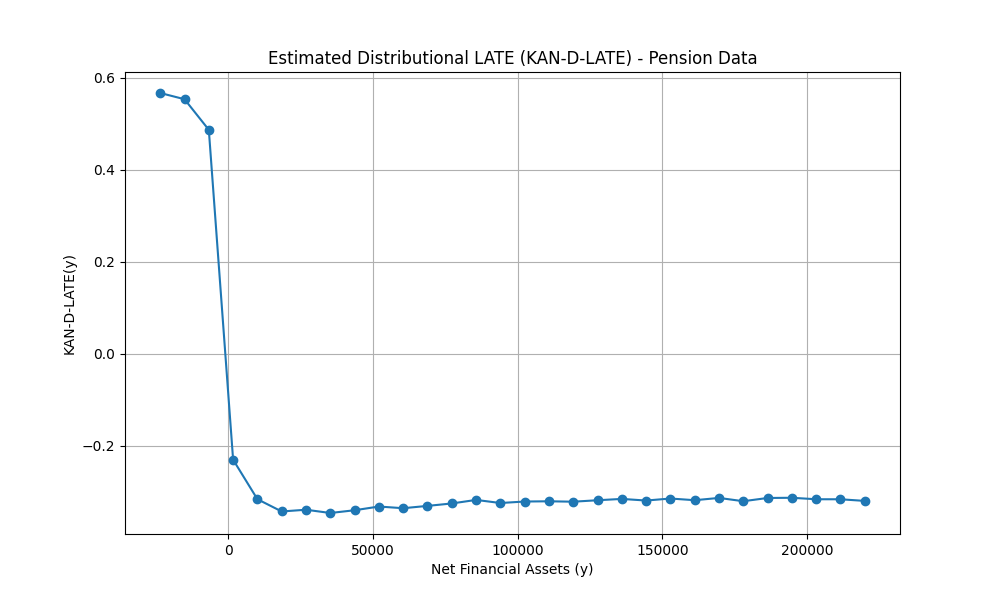
\includegraphics[width=0.5\textwidth]{empirical_kan-d-iv-late_plot.png}\label{fig:kan_empirical}}
    
    \vspace{1em} % Add some vertical space between subfigures
    
    \subfigure[Random Forest-based D-IV-LATE]{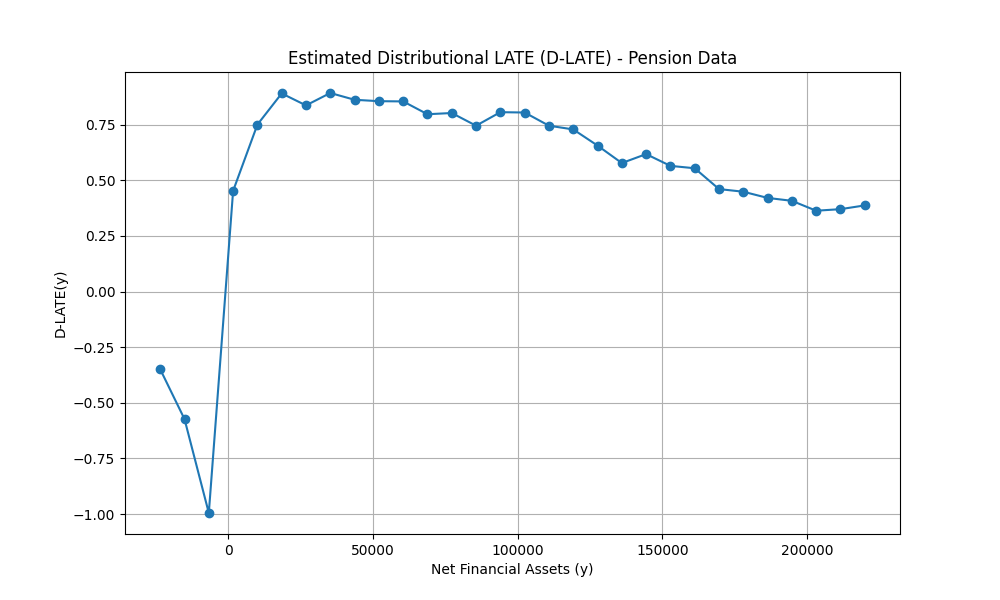
\includegraphics[width=0.5\textwidth]{empirical_rf-d-iv-late_plot.png}\label{fig:rf_empirical}}
    \caption{Comparison of Estimated D-IV-LATE of 401(k) Participation on Net Financial Assets using KANs (Top) and Random Forests (Bottom) for nuisance functions. The plots show $\hat{\Delta}(y) = \hat{\mathbb{P}}(Y(1) \le y | \text{compliers}) - \hat{\mathbb{P}}(Y(0) \le y | \text{compliers})$ against $y$ (net financial assets).}
    \label{fig:empirical_dlate_comparison}
\end{figure}

\textbf{Random Forest D-IV-LATE Results (Bottom Panel, Figure \ref{fig:empirical_dlate_comparison}).}
The findings for the RF-based estimator indicated that for very low levels of net financial assets (e.g., $y \approx -\$23k \text{ to } -\$6k$), the D-IV-LATE is negative (ranging from -0.35 to -0.99). This suggests that, for compliers, 401(k) participation reduces the probability of having extremely low or negative net financial assets. As $y$ increases into positive territory, the D-IV-LATE becomes positive, peaking at approximately 0.89 around $y \approx \$18.5k$. This indicates an increased probability of compliers' assets being below these moderate positive thresholds if they participate, consistent with wealth shifting towards these levels. For higher $y$ values (e.g., above \$120k), the D-IV-LATE estimates remain positive but generally decrease.

\textbf{KAN-D-IV-LATE Results (Top Panel, Figure \ref{fig:empirical_dlate_comparison}).}
The KAN-based estimator revealed a strikingly different pattern, particularly at the lower tail. For very low net financial assets, the KAN D-IV-LATE is positive and large (approx. 0.57 at the lowest $y$). This suggests that for compliers, 401(k) participation *increases* the probability of their assets falling at or below these very low levels. As $y$ increases towards zero, the KAN D-IV-LATE falls sharply, becoming negative around $y = 1,724$. For positive $y$ values, the KAN D-IV-LATE is negative and relatively stable (around -0.32), indicating that participation *decreases* the probability of wealth being at or below these positive thresholds. This latter part is consistent with a rightward shift in the wealth distribution for most compliers.

%\textbf{Comparative Discussion.}
A comparison shows the divergence between the two estimators is most pronounced at the lower tail of the wealth distribution. The RF-based estimator suggests a protective effect of 401(k) participation against very low wealth. In contrast, the KAN-based estimator suggests a counter-intuitive accentuation of the extreme lower tail for compliers. This highlights that the choice of ML model for nuisance functions can lead to substantially different qualitative conclusions about treatment effect heterogeneity.

The KAN results, if reflecting a genuine phenomenon, could imply complex financial adjustments among low-wealth compliers upon 401(k) participation (e.g., taking on debt, liquidating other small assets). Conversely, if the KAN result is an artefact of model instability in sparse data regions, the RF estimate might be a more robust, albeit potentially over-smoothed, representation. Distinguishing these possibilities requires further investigation (e.g., robustness checks, examination of covariate overlap).

These differing distributional insights are richer than what a single LATE point estimate would provide. The comparison underscores the central theme of this paper: the choice of nuisance function estimator is critical. While the RF-based results align more with conventional expectations of 401(k) effects (e.g., \citet{chernozhukov2004impact}), the KAN-based results, by potentially capturing more complex non-linearities, challenge these interpretations and suggest that the impact of 401(k) participation might be more nuanced than previously understood, especially for vulnerable subgroups. This motivates the "caveat emptor" discussed in Section \ref{sec:caveat_emptor}.

Confidence intervals for these D-IV-LATE curves are essential for formal inference and assessing the statistical significance of these patterns and divergences. Developing robust methods for these, suitable for complex multi-stage estimators, is an important area for future research.

\section{Caveat Emptor The Role of Nuisance Function Estimators and Model Choice}
\label{sec:caveat_emptor}

The comparative empirical results presented in Section \ref{sec:empirical_app}, particularly the divergence in estimated D-IV-LATE curves for 401(k) participation (Figure \ref{fig:empirical_dlate_comparison}), underscore a critical message for applied researchers: the choice of machine learning model for nuisance function estimation within the DML framework is not a mere implementation detail but a decision that can have profound implications for substantive conclusions. This section elaborates on this "caveat emptor" (buyer beware) principle.

The DML framework's promise of Neyman orthogonality provides robustness against first-order errors in nuisance function estimation, allowing for $\sqrt{n}$-consistent estimation of the target parameter even when using flexible ML models. However, this theoretical protection does not render the choice of ML model irrelevant. Higher-order biases, finite-sample performance, and the ability to accurately approximate the true underlying nuisance functions can still differ substantially across ML methods.

Our empirical application illustrates this point. The Random Forest-based D-IV-LATE estimator produced results for the 401(k) data that might be considered more aligned with prior expectations or simpler theories of wealth accumulation—primarily a protective effect at the lower tail and a shift towards moderate positive wealth. In contrast, the KAN-based estimator, with its potentially greater flexibility in capturing complex non-linearities via learnable spline activations, suggested a more intricate pattern: an adverse effect at the very lowest end of the wealth distribution, followed by a strong positive shift.

This divergence raises several important considerations.
First, regarding model flexibility and true nuisance functions, if the true nuisance functions ($\mu(y,w,x)$, $p(z,x)$, $\pi(x)$) possess complex, highly localised non-linearities, a more adaptive and flexible model like KANs might be better equipped to approximate them accurately. Less flexible models, or models with different inductive biases (like the averaging nature of Random Forests), might smooth over these nuances, leading to a potentially distorted view of the D-IV-LATE. The superior performance of KANs in our DGP 2 (Section \ref{subsec:sim_dgp2}), which was designed with such complexities, lends credence to this.
Second, concerning sensitivity in sparse data regions, highly flexible models can sometimes be sensitive in regions of sparse data, potentially fitting noise or exhibiting instability. The counter-intuitive findings from KANs at the extreme lower tail of the wealth distribution in the 401(k) application could, in part, reflect such challenges if covariate overlap or data density is low in that region for the complier subpopulation. This necessitates careful diagnostic checks and robustness analyses when using highly adaptive methods.
Third, there is an interpretability versus accuracy trade-off. While KANs may offer greater accuracy in approximating complex functions, their internal workings can be less transparent than, for example, a Random Forest where feature importance measures are readily available. Researchers must weigh the potential gains in estimation accuracy against the interpretability of the nuisance models themselves, although the DML framework's primary goal is accurate estimation of the causal parameter, not necessarily interpretation of nuisance parts.
Fourth, computational cost is a factor. More flexible or complex models like KANs can also come with higher computational costs, especially within a cross-fitting procedure repeated for many $y$-values in DTE estimation. This is a practical consideration in model selection.
Finally, there is the matter of theoretical assumptions versus practical performance. While DML theory relies on certain convergence rates and Donsker properties for nuisance estimators (Assumption \ref{ass:regularity_merged}), verifying these for any given ML model in a finite sample with specific data is non-trivial. The empirical performance observed in simulations and applications becomes a crucial guide. Our findings suggest that KANs are a promising candidate for satisfying these conditions in complex settings, but like all ML methods, their application requires care.

The "caveat emptor" here is not to distrust flexible ML models in causal inference, but rather to approach their use with a critical and informed perspective. Researchers should be aware that their choice of nuisance estimator can matter significantly for the results. Whenever possible, they should conduct sensitivity analyses using different well-motivated ML models for nuisance functions. If results diverge substantially, this signals a need for deeper investigation into the data structure and model assumptions. They should also carefully consider the theoretical properties of the chosen ML models in relation to the DML framework's requirements. Furthermore, it is important to pay attention to regions of the data (e.g. tails of distributions, areas with poor covariate overlap) where flexible models might behave unexpectedly. Finally, researchers should report transparently on the ML models used, their tuning, and any sensitivity analyses performed.

Ultimately, the goal is to leverage the power of modern machine learning to obtain more credible and nuanced causal estimates. This requires not only sophisticated statistical frameworks like DML but also a thoughtful and critical approach to the implementation of the machine learning components themselves. The KAN-D-IV-LATE estimator represents one step in this direction, offering enhanced capabilities but also reinforcing the need for careful application and interpretation.

\section{Conclusion}
\label{sec:conclusion}

This paper has explored the estimation of Distributional Instrumental Variable Local Average Treatment Effects (D-IV-LATE), a critical parameter for understanding the full impact of endogenous treatments. We have detailed and compared two DML-based estimation approaches. One employs standard machine learning models like Random Forests for nuisance function estimation, and the other is a novel KAN-D-IV-LATE estimator that leverages the approximation power of Kolmogorov-Arnold Networks.

Our theoretical discussion highlighted the DML framework's robustness to regularisation bias and established the asymptotic normality for D-IV-LATE estimators, contingent on nuisance estimators meeting certain regularity conditions. We argued that KANs, due to their architectural design and approximation properties, are a promising candidate for satisfying these conditions, especially in complex, non-linear settings.

Monte Carlo simulations demonstrated that while standard ML-based D-IV-LATE estimators can perform well, the KAN-D-IV-LATE estimator exhibited superior performance, particularly lower RMSE, when nuisance functions were characterised by intricate non-linearities. This suggests KANs' potential for more accurate nuisance function estimation translates into more reliable D-IV-LATE estimates.

The empirical application to the 401(k) SIPP dataset provided a stark illustration of how the choice of nuisance function estimator can impact substantive findings. The RF-based and KAN-based D-IV-LATE estimators yielded notably different distributional impact curves for 401(k) participation on net financial assets, especially at the lower tail of the wealth distribution. While the RF-based estimator suggested a protective effect, the KAN-based estimator pointed to a more complex, counter-intuitive pattern, potentially increasing the probability of very low wealth for compliers. These divergent results underscore our central "caveat emptor". The selection of ML models for nuisance components in DML is a critical research choice, not a mere implementation detail, and can significantly shape policy-relevant conclusions.

Despite the contributions, our approach shares the inherent limitations of the IV framework, such as reliance on instrument credibility and potential issues with weak instruments. Furthermore, the very flexibility that makes KANs appealing can also lead to challenges in sparse data regions or require careful tuning.

This research opens several promising avenues for future work. Developing robust weak-instrument inference procedures tailored for D-IV-LATE, particularly with highly flexible nuisance estimators like KANs, is crucial. Extending the D-IV-LATE framework to accommodate continuous treatments, multiple instruments, or dynamic settings would also greatly enhance its applicability. Further investigation into optimal KAN architectures and hyperparameter tuning strategies within the DML context is warranted.

In conclusion, the D-IV-LATE estimators discussed provide valuable tools for a deeper understanding of causal effects. The comparative analysis, especially with the introduction of KAN-D-IV-LATE, emphasises that while DML offers a powerful framework, the careful selection, implementation, and validation of the underlying machine learning models for nuisance functions are paramount for credible and nuanced causal inference.





\vskip 0.2in
\begin{thebibliography}{99}
\bibitem[Abadie(2002)]{abadie2002bootstrap} Abadie, A. (2002). Bootstrap tests for distributional treatment effects in instrumental variable models. \textit{Journal of the American statistical Association}, 97(457), 284-292.
\bibitem[Angrist et al.(1996)]{angrist1996identification} Angrist, J. D., Imbens, G. W., \& Rubin, D. B. (1996). Identification of causal effects using instrumental variables. \textit{Journal of the American statistical Association}, 91(434), 444-455.
\bibitem[Athey et al.(2019)]{athey2019generalized} Athey, S., Tibshirani, J., \& Wager, S. (2019). Generalized random forests. \textit{The Annals of Statistics}, 47(2), 1148-1178. % Placeholder - please verify
\bibitem[Belloni et al.(2014)]{belloni2014high} Belloni, A., Chernozhukov, V., \& Hansen, C. (2014). Inference on treatment effects after selection among high-dimensional controls. \textit{The Review of Economic Studies}, 81(2), 608-650.
\bibitem[Bickel et al.(1993)]{bickel1993efficient} Bickel, P. J., Klaassen, C. A., Ritov, Y., \& Wellner, J. A. (1993). \textit{Efficient and adaptive estimation for semiparametric models}. Springer.
\bibitem[Byambadalai et al.(2024)]{byambadalai24a} Byambadalai, U., Oka, T., \& Yasui, S. (2024). Estimating distributional treatment effects in randomised experiments: Machine learning for variance reduction. In \textit{International Conference on Machine Learning} (pp. 5082-5113). PMLR.
\bibitem[Chen(2024)]{chen2025gpkan} Chen, A. S. (2024). GP-KAN: Gaussian Process Kolmogorov-Arnold Networks. \textit{arXiv preprint arXiv:2407.18397}.
\bibitem[Chernozhukov \& Hansen(2004)]{chernozhukov2004impact} Chernozhukov, V., \& Hansen, C. (2004). The impact of 401 (k) participation on the wealth distribution: an instrumental quantile regression analysis. \textit{The Review of Economic Studies}, 71(3), 735-764.
\bibitem[Chernozhukov et al.(2013)]{chernozhukov2013inference} Chernozhukov, V., Fern{\'a}ndez-Val, I., \& Melly, B. (2013). Inference on counterfactual distributions. \textit{Econometrica}, 81(6), 2205-2268.
\bibitem[Chernozhukov et al.(2018)]{chernozhukov2018debiased} Chernozhukov, V., Chetverikov, D., Demirer, M., Duflo, E., Hansen, C., Newey, W., \& Robins, J. (2018). Double/debiased machine learning for treatment and structural parameters. \textit{The Econometrics Journal}, 21(1), C1-C68.
\bibitem[Doksum(1974)]{doksum1974empirical} Doksum, K. (1974). Empirical probability plots and statistical inference for nonlinear models in the two-sample case. \textit{The annals of statistics}, 267-277.
\bibitem[Firpo(2007)]{firpo2007efficient} Firpo, S. (2007). Efficient semiparametric estimation of quantile treatment effects. \textit{Econometrica}, 75(1), 259-276.
\bibitem[Hoagland(2020)]{hoagland2020who} Hoagland, A. (2020). \textit{Who Do Innovations Reach? The Influence of Trainings on Mental Health Treatments}. Working Paper.
\bibitem[Imbens \& Angrist(1994)]{imbens1994} Imbens, G. W., \& Angrist, J. D. (1994). Identification and estimation of local average treatment effects. \textit{Econometrica}, 62(2), 467-475.
\bibitem[Imbens \& Rubin(1997)]{imbens1997estimating} Imbens, G. W., \& Rubin, D. B. (1997). Estimating outcome distributions for compliers in instrumental variables models. \textit{The Review of Economic Studies}, 64(4), 555-574.
\bibitem[Kallus \& Oprescu(2023)]{kallus2023robust} Kallus, N., \& Oprescu, M. (2023). Robust and agnostic learning of conditional distributional treatment effects. In \textit{International Conference on Artificial Intelligence and Statistics} (pp. 6037-6060). PMLR.
\bibitem[Koenker et al.(2017)]{koenker2017handbook} Koenker, R., Chernozhukov, V., He, X., \& Peng, L. (2017). \textit{Handbook of quantile regression}. CRC press.
\bibitem[Koenker(2005)]{koenker2005quantile} Koenker, R. (2005). \textit{Quantile regression} (Vol. 38). Cambridge university press.
\bibitem[Kratsios \& Furuya(2025)]{kratsios2025kolmogorov} Kratsios, A., \& Furuya, T. (2025). Kolmogorov-Arnold Networks: Approximation and Learning Guarantees for Functions and their Derivatives. \textit{arXiv preprint arXiv:2504.15110}.
\bibitem[Lehmann \& D'Abrera(1975)]{lehmann1975nonparametrics} Lehmann, E. L., \& D'Abrera, H. J. (1975). \textit{Nonparametrics: statistical methods based on ranks}. Holden-day.
\bibitem[Liu et al.(2024)]{liu2024kan} Liu, Z., Wang, Y., Vaidya, S., Ruehle, F., Halverson, J., Solja{\v{c}}i{\'c}, M., ... \& Tegmark, M. (2024). Kan: Kolmogorov-arnold networks. \textit{arXiv preprint arXiv:2404.19756}.
\bibitem[Mehendale et al.(2025)]{mehendale2025kanite} Mehendale, E., Thorat, A., Kolla, R., \& Pedanekar, N. (2025). KANITE: Kolmogorov-Arnold Networks for ITE estimation. \textit{arXiv preprint arXiv:2503.13912}.
\bibitem[Newey(1994)]{newey1994asymptotic} Newey, W. K. (1994). The asymptotic variance of semiparametric estimators. \textit{Econometrica: Journal of the Econometric Society}, 1349-1382.
\bibitem[Newey(1997)]{newey1997convergence} Newey, W. K. (1997). Convergence rates and asymptotic normality for series estimators. \textit{Journal of Econometrics}, 79(1), 147-168. % Placeholder - please verify
\bibitem[Peng et al.(2022)]{peng2022rates} Peng, W., Coleman, T. and Mentch, L. (2022). Rates of convergence for random forests via generalised U-statistics. \textit{Electronic Journal of Statistics}, 16(1), pp.232-292. % Placeholder - please verify

\bibitem[Wager and Athey(2015)]{wager2015adaptive} Wager, S., \& Athey, S. (2015). Adaptive Causal Inference. \textit{arXiv preprint arXiv:1503.02300}. % Placeholder for actual publication if available, e.g., PNAS. Please verify.


\end{thebibliography}

\end{document}
